
\documentclass[addpoints]{exam}

% https://tex.stackexchange.com/questions/66154/how-to-construct-a-coloured-box-with-rounded-corners
% \usepackage{tcolorbox}

\usepackage{dashbox}
\usepackage{listings}
\usepackage{mdframed}
\usepackage{xcolor}
\usepackage{csquotes}

\usepackage{tikz}
\usetikzlibrary{automata, positioning}

\definecolor{light-gray}{gray}{0.89}

\firstpageheader{LOAL}{Automata Exercises}{2020}

% \firstpagefooter{}{\textbf{Exam continues on next page}}{Page \thepage\ of \numpages}
\firstpagefooter{}{}{Page \thepage\ of \numpages}
% \firstpagefooter{}{Page \thepage\ of \numpages}
% Footer after the first page
\runningfooter{}{}{Page \thepage\ of \numpages}

% Lower the footer a bit
\extrafootheight{-0.3cm}

% Draw a box around the points of a question
\boxedpoints
\bonuspointformat{\dbox{\thepoints}}

% Define how bonus points are labelled
\bonuspointpoints{bonus point}{bonus points}

\totalformat{\fbox{Points for question \thequestion: \totalpoints}}
\bonustotalformat{\dbox{Bonus points for question \thequestion: \totalbonuspoints}}

\newcommand{\labeledThreeStateAutomaton}{
 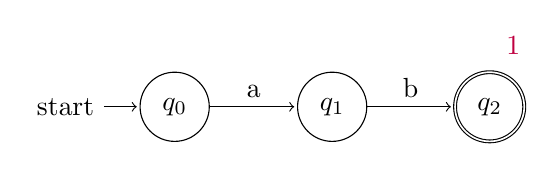
\begin{tikzpicture}[shorten >=1pt,node distance=2cm,on grid,auto]
   \node[state, initial] (q0) {$q_0$};
   \node[state] (q1) [right=of q0] {$q_1$};
   \node[state, accepting, label={[purple, shift={(0.3, 0.08)}] 1 }] (q2) [right=of q1] {$q_2$};
   \path[->]
    (q0) edge node {a} (q1)
    (q1) edge node {b} (q2);
 \end{tikzpicture}
}
\newcommand{\labeledAutomatonWithTrapStates}{
 \begin{tikzpicture}[shorten >=1pt,node distance=3cm,on grid,auto]
   \node[state, initial] (q0) {$q_0$};
   \node[state] (q1) [right=of q0] {$q_1$};
   \node[state, accepting, label={[purple, shift={(0.3, 0.08)}] \fbox{1} }] (q2) [right=of q1] {$q_2$};
   \node[state] (q3) [below =of q1] {$q_3$};
   \path[->]
    (q0) edge node {a} (q1)
         edge node [swap] {b} (q3)
    (q1) edge node {b} (q2)
         edge node {a} (q3)
    (q2) edge [loop below] node {a|b} ()
    (q3) edge [loop below] node {a|b} ();
 \end{tikzpicture}
}

\begin{document}

\begin{center}
  \fbox{\fbox{\parbox{5.5in}{\centering
  Answer the questions on a sheet of paper, either on this one or use your own sheet of paper with your name on it. Begin each of your answers with the question number.
  }}}
\end{center}

% \begin{itemize}
%     % \item Duration: 45 minutes
%     % \item Total points: \numpoints
%   \item You're not allowed to use material like your lecture notes or the lecture slides.
%   \item Remember: This exam makes up $33.\overline{3}$\% of your semester grade in LOAL.
%   \item Lesen Sie sich die Fragen in Ruhe durch. Sollten Sie eine Frage nicht verstehen, fragen Sie sofort.
% \end{itemize}

% \vspace{.1in}
\makebox[\textwidth]{Your name:\enspace\hrulefill}
\vspace{.2in}

\begin{questions}
  \question Add the name of each element of the automata
  \droptotalpoints

  \labeledAutomatonWithTrapStates

  \begin{parts}
    \part
    \textcolor{purple}{\fbox{1}}: trap state
    \part
    \textcolor{purple}{\fbox{2}}:
    \part
    \textcolor{purple}{\fbox{3}}:
  \end{parts}
  Possible labels: \enquote{transition}, \enquote{final state}, \enquote{grammar}, \enquote{alphabet}, \enquote{trap state}


%   \question Translate these formulas from predicate logic to English:
%   \droptotalpoints
%   \droptotalbonuspoints
%
%   \begin{parts}
%
%     \part[5]
%     $\forall x: isDuck(x) \lor isPenguin(x) \Rightarrow isBird(x)$
%
%     \part[5]
%     $\forall x: isPerson(x) \Rightarrow \lnot knowsEverything(x)$
%
%     \part [5]
%     $\exists x: isVehicle(x) \land isBus(x)$
%
%     \part[5]
%     $\lnot \exists x: isMonkey(x) \land isFish(x)$
%
%     \bonuspart[10]
%     $\forall x \exists y: isSomeone(x) \Rightarrow isAfraidOf(x, y)$
%
%   \end{parts}
%
%
%   \vspace{.2in}
%
%
%   \question Translate these English sentences to predicate logic:
%   \droptotalpoints \droptotalbonuspoints
%   \begin{parts}
%
%     \part[5]
%     All students have to write exams.
%     \part[5]
%     I don't like hamburgers.
%     % \part[5]
%     % There are sunny days in December.
%     \part[5]
%     Nobody has set foot on Venus.
%     \part[5]
%     Some people are very kind.
%     \bonuspart[10]
%     % $\forall x \exists y: isSuperHeroMovie(x) \Rightarrow isPerson(y) \land likes(y, x)$
%     Some people like all super hero movies.
%
%   \end{parts}
%
%   \newpage
%
%   \question
%   Consider the following Prolog program:
%   \droptotalpoints
%
%     \begin{mdframed}[ frametitle=miaFood.pl, frametitlerule=true, frametitlebackgroundcolor=light-gray!30, backgroundcolor=light-gray, roundcorner=2pt, leftmargin=1, rightmargin=1, innerleftmargin=5, innertopmargin=5, innerbottommargin=5, outerlinewidth=2, linecolor=gray ]
%
%       \begin{lstlisting}[
%         language=Prolog,
%         basicstyle=\ttfamily,
%         keywordstyle=\textbf
%       ]
% likes(mia, Food) :- isItalian(Food).
% likes(mia, Food) :- isAmerican(Food),
%                     isVegetarian(Food).
% isItalian(pizza).
% isItalian(lasagna).
% isItalian(spaghetti).
% isAmerican(frenchFries).
% isAmerican(hotDog).
% isVegetarian(frenchFries).
%       \end{lstlisting}
%     \end{mdframed}
%
%     When writing a Prolog query, make it clear which letters are uppercase and which are lowercase.
%
%   \begin{parts}
%     \part[10]
%     Based on the program's rules, describe what kind of food Mia likes.
%     \part[5]
%     Does Mia like hot dogs?
%     \part[5]
%     Write a Prolog query that tells you whether Mia likes pizza.
%     \part[5]
%     Write a Prolog query that tells you which food Mia likes.
%     \part[5]
%     Write a Prolog query that tells you who likes spaghetti.
%   \end{parts}

\end{questions}

% Put the grade table at the bottom of the page
% \vspace*{\fill}
% \hrulefill
% \begin{center}
%   \combinedgradetable[h]
% \end{center}

\end{document}

